%=========================================================================
% (c) Radim Loskot, 2012

\chapter{Úvod}
\chapter{QR kódy}

\begin{figure}[H]
  \begin{center}
    \scalebox{0.20}{
      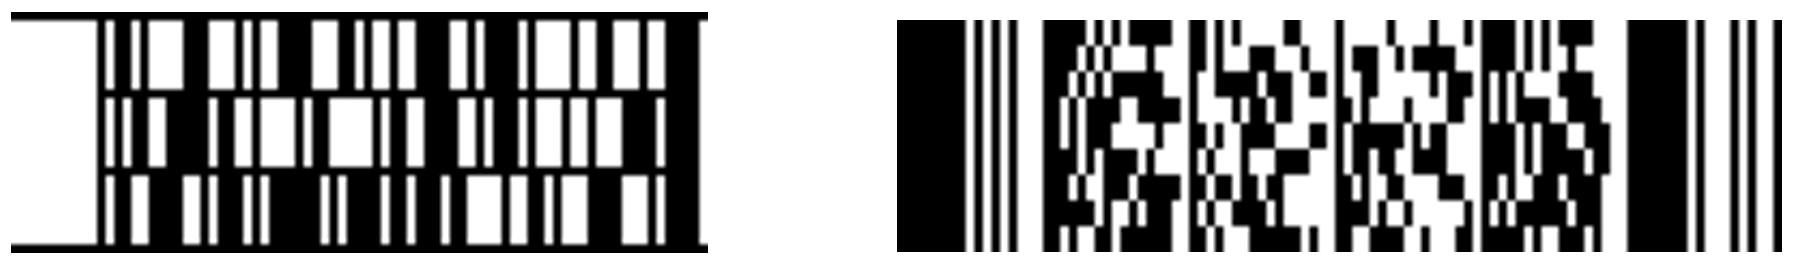
\includegraphics{fig/stackedCodes.PNG}
    } 
    \caption{Skládané dvourozměrné kódy -- Code 49 (vlevo) a PDF417 (vpravo)}
    \label{stackedCodes}
  \end{center}
\end{figure}

\begin{figure}[H]
  \begin{center}
    \scalebox{0.20}{
      
\includegraphics{fig/matrixCodes.PNG}
    } 
    \caption{Maticové dvourozměrné kódy -- Data Matrix, Aztec Code a MaxiCode}
    \label{matrixCodes}
  \end{center}
\end{figure}

\begin{figure}[H]
  \begin{center}
    \scalebox{0.20}{
      
\includegraphics{fig/corruptedQRCodes.PNG}
    } 
    \caption{Ukázka poškozených, ale opravitelných QR kódů}
    \label{corruptedQRCodes}
  \end{center}
\end{figure}

\begin{figure}[H]
  \begin{center}
    \scalebox{0.20}{
      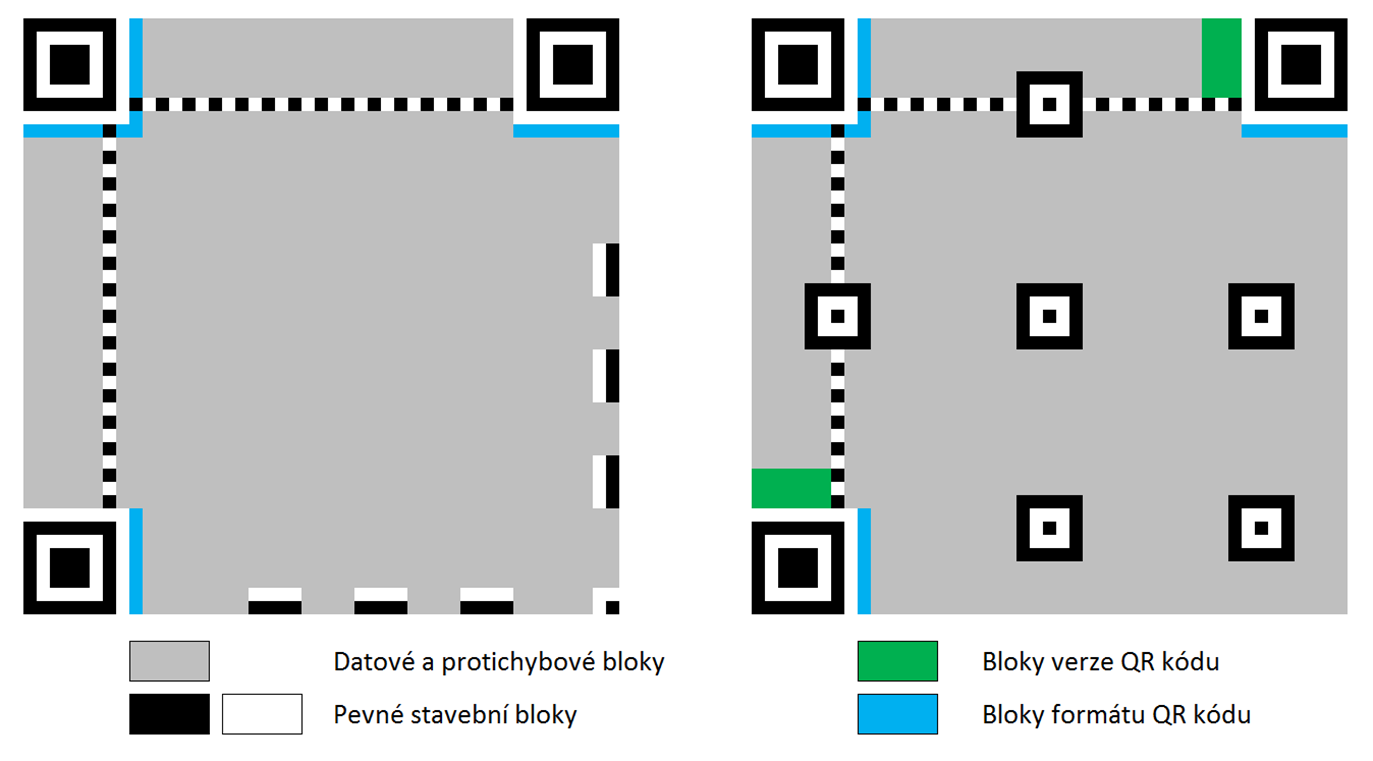
\includegraphics{fig/QRCodeModel12Comparision.PNG}
    } 
    \caption{Porovnaní QR kódu stejné verze modelu 1 (vlevo) a modelu 2 (vpravo)}
    \label{QRCodeModel12Comparision}
  \end{center}
\end{figure}

\begin{figure}[H]
  \begin{center}
    \scalebox{0.15}{
      
\includegraphics{fig/microQRIntroducion.PNG}
    } 
    \caption{Micro QR kód}
    \label{microQRIntroducion}
  \end{center}
\end{figure}

\begin{figure}[H]
  \begin{center}
    \scalebox{0.30}{
      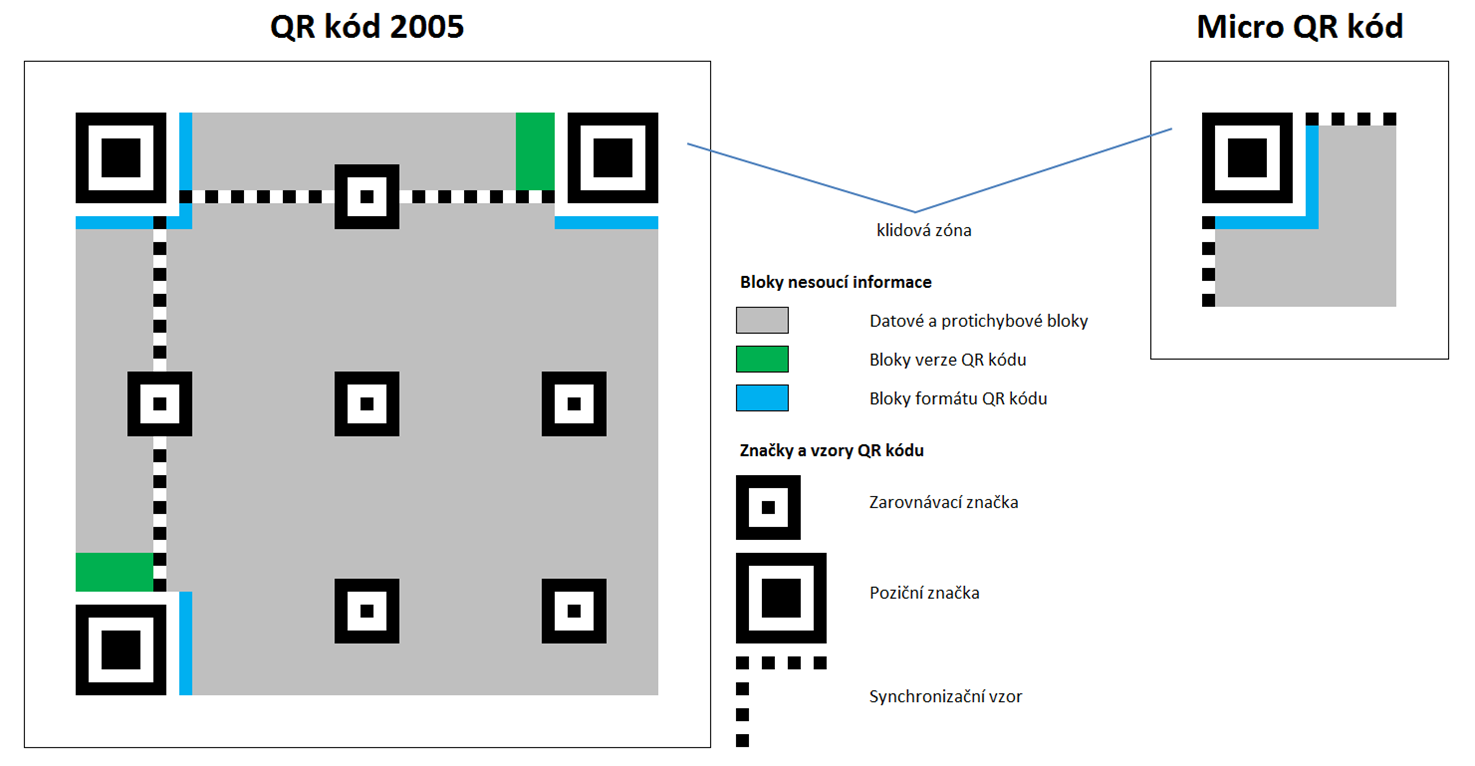
\includegraphics{fig/QRCodesStructure.PNG}
    } 
    \caption{Struktura QR kódu 2005 (znázorněna verze 7)}
    \label{QRCodesStructure}
  \end{center}
\end{figure}

\begin{figure}[H]
  \begin{center}
    \scalebox{0.15}{
      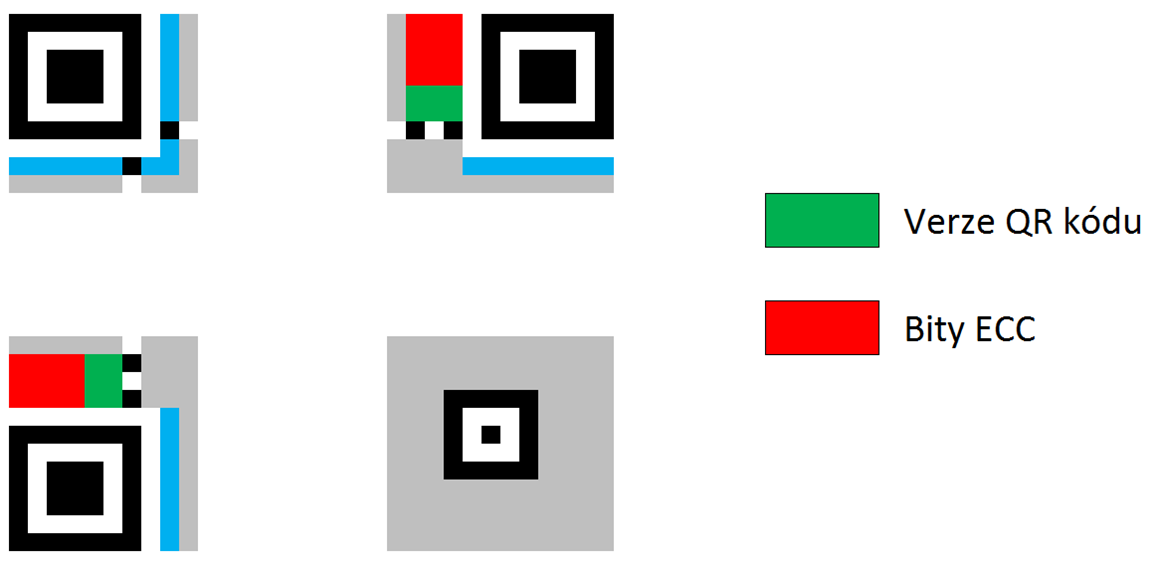
\includegraphics{fig/QRCodeVersionMetainformation.PNG}
    } 
    \caption{Znázornění bloku s metainformací verze QR kódu}
    \label{QRCodeVersionMetainformation}
  \end{center}
\end{figure}

\begin{figure}[H]
  \begin{center}
    \scalebox{0.15}{
      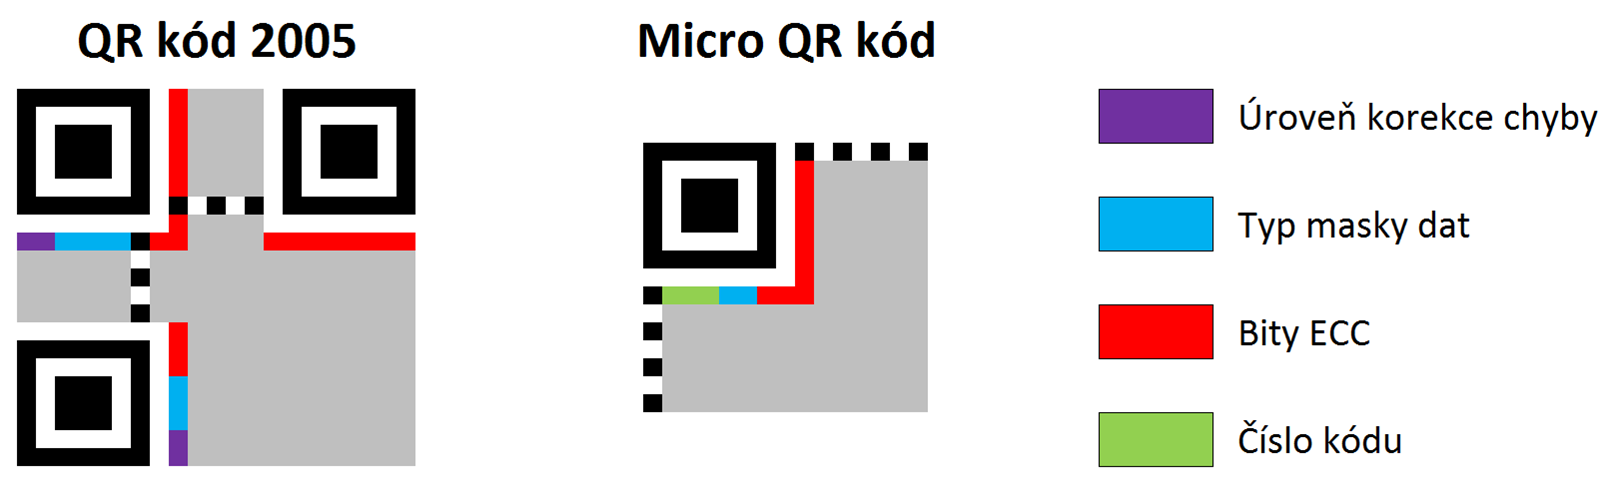
\includegraphics{fig/QRCodeFormatMetainformation.PNG}
    } 
    \caption{Znázornění bloku s metainformací formátu QR kódu}
    \label{QRCodeFormatMetainformation}
  \end{center}
\end{figure}

\begin{figure}[H]
  \begin{center}
    \scalebox{0.25}{
      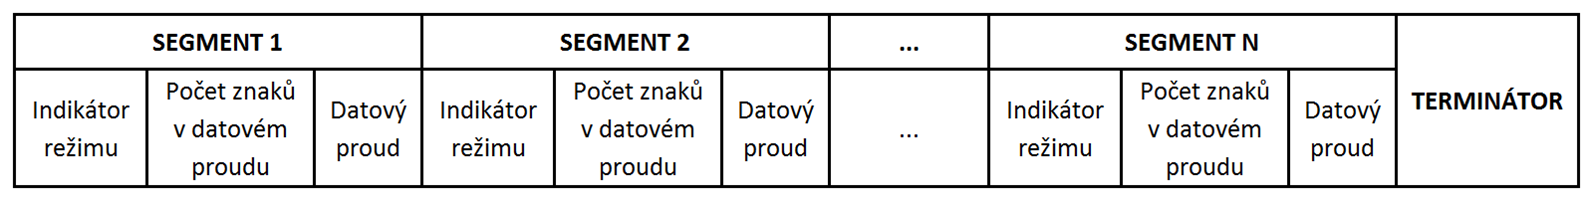
\includegraphics{fig/QRCodeDataSegments.PNG}
    } 
    \caption{Ukázka kódování dat do datových segmentů}
    \label{QRCodeDataSegments}
  \end{center}
\end{figure}

\begin{figure}[H]
  \begin{center}
    \scalebox{0.18}{
      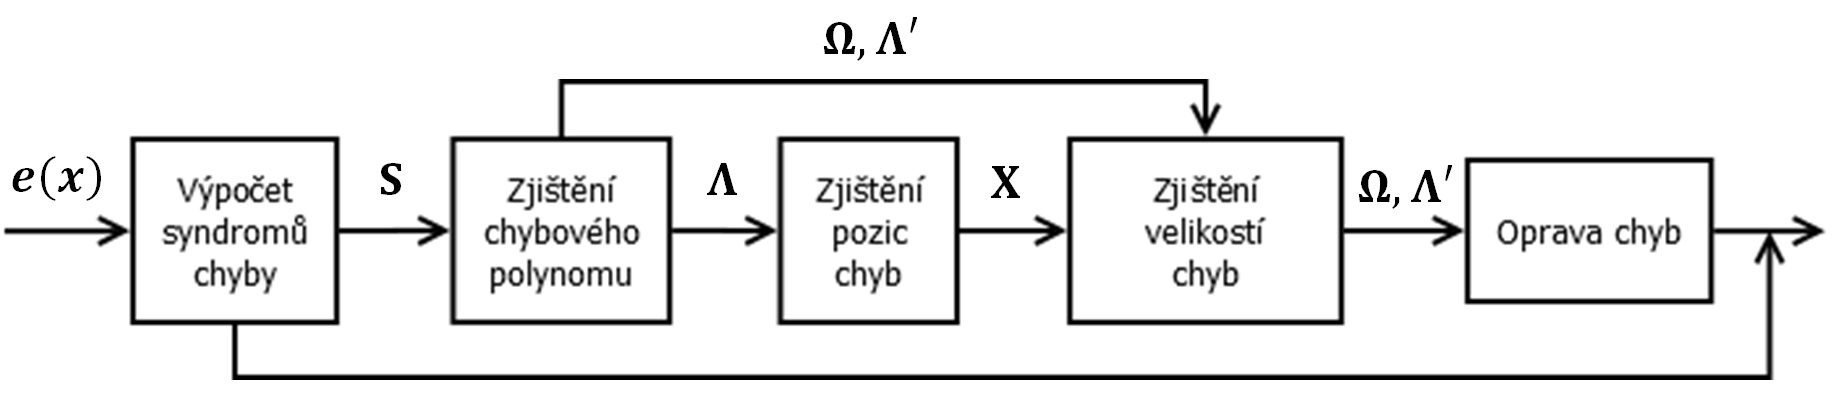
\includegraphics{fig/ReedSolomonDecodingProcess.PNG}
    } 
    \caption{Proces dekódování Reed Solomon kódu}
    \label{ReedSolomonDecodingProcess}
  \end{center}
\end{figure}

\begin{figure}[H]
  \begin{center}
    \scalebox{0.40}{
      
\includegraphics{fig/CreatingOutputPatternProcess.PNG}
    } 
    \caption{Kroky vedoucí ke tvorbě výstupního vzoru}
    \label{CreatingOutputPatternProcess}
  \end{center}
\end{figure}

\begin{figure}[H]
  \begin{center}
    \scalebox{0.35}{
      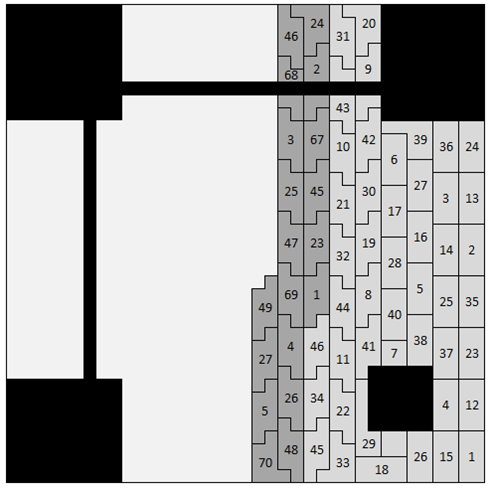
\includegraphics{fig/PuttingDataCodewordsIntoQRCode.PNG}
    } 
    \caption{Znázornění způsobu organizace kódových slov v QR kódu}
    \label{PuttingDataCodewordsIntoQRCode}
  \end{center}
\end{figure}

\begin{figure}[H]
  \begin{center}
    \scalebox{0.15}{
      
\includegraphics{fig/QRCodeDataMasks.PNG}
    } 
    \caption{Sada datových masek QR kódu}
    \label{QRCodeDataMasks}
  \end{center}
\end{figure}

\begin{figure}[H]
  \begin{center}
    \scalebox{0.20}{
      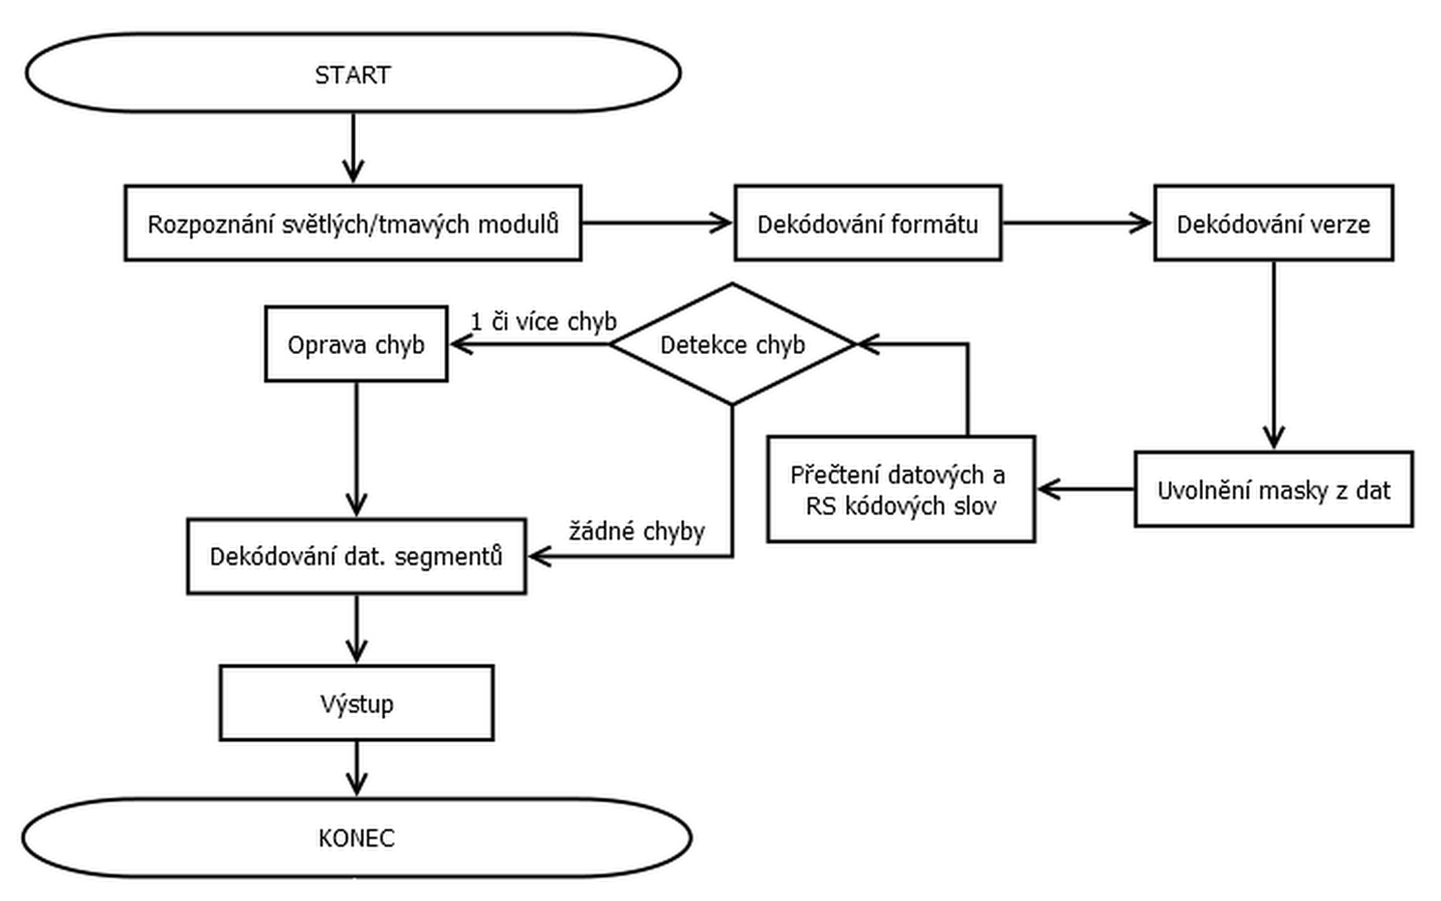
\includegraphics{fig/QRCodeReferenceReadingProcess.PNG}
    } 
    \caption{Referenční vývojový diagram znázorňující kroky čtení QR kódu}
    \label{QRCodeReferenceReadingProcess}
  \end{center}
\end{figure}

\begin{equation}
  F = \{ 0, 1, \alpha^1, \alpha^2, \ldots, \alpha^{2^{m}-2}, \alpha^{2^{m}-1},
  \alpha^{2^{m}}\}
\end{equation}

\begin{equation}
  f(x) = f_{0} + f_{1}x + f_{2}x^2 + \ldots + f_{n-1}x^{n-1}
\end{equation}

\begin{equation}
  \frac{f(x) x^{n-k}}{g(x)} = h(x) + \frac{r(x)}{g(x)}
\end{equation}

\begin{equation}
  \mathbf{G} = \left(
    \begin{array}{ccccccccc}
      g_{n-k} & g_{n-k-1} & \ldots & g_{1} & g_{0} & 0 & 0 & \ldots & 0 \\
      0 & g_{n-k} & g_{n-k-1} & \ldots & g_{1} & g_{0} & 0 & \ldots & 0 \\
      \vdots & \vdots & \vdots & \vdots & \ddots & \vdots & \vdots & \vdots &
      \vdots\\
      0 & 0 & \ldots & 0 & g_{n-k} & g_{n-k-1} & \ldots & g_{1} & g_{0} \\
    \end{array}
  \right)
\end{equation}

\begin{equation}
  t \leq \frac{n - k}{2}
\end{equation}

\begin{equation}
  0 < k < n < 2^{m} + 2
\end{equation}
\chapter{Google Android}

\begin{figure}[H]
  \begin{center}
    \scalebox{0.30}{
      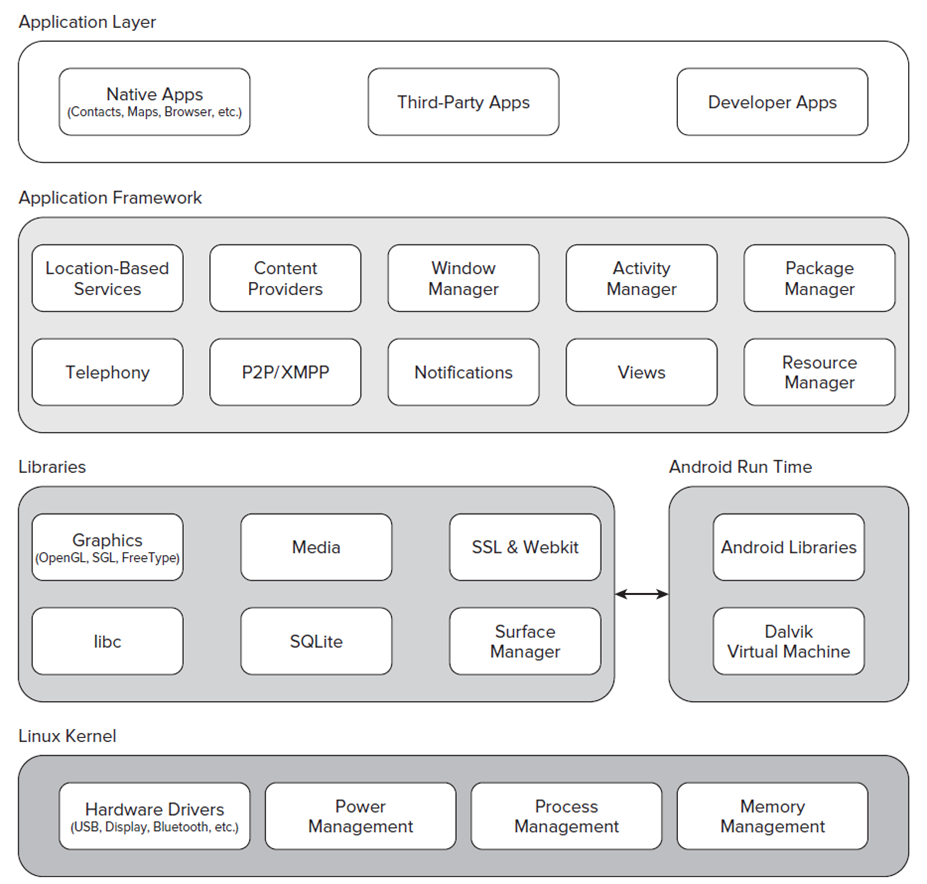
\includegraphics{fig/AndroidArchitecture.PNG}
    } 
    \caption{Architektura platformy Android}
    \label{AndroidArchitecture}
  \end{center}
\end{figure}

\chapter{Návrh}

\begin{figure}[H]
  \begin{center}
    \scalebox{0.15}{
      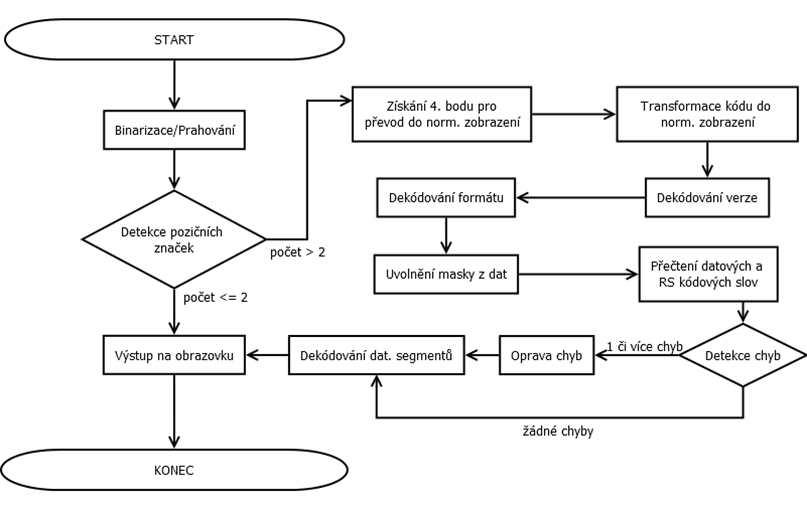
\includegraphics{fig/QRCodeReadingProcess.PNG}
    } 
    \caption{Vývojový diagram navrženého postupu pro čtení QR kódů}
    \label{QRCodeReadingProcess}
  \end{center}
\end{figure}

\begin{figure}[H]
  \begin{center}
    \scalebox{0.15}{
      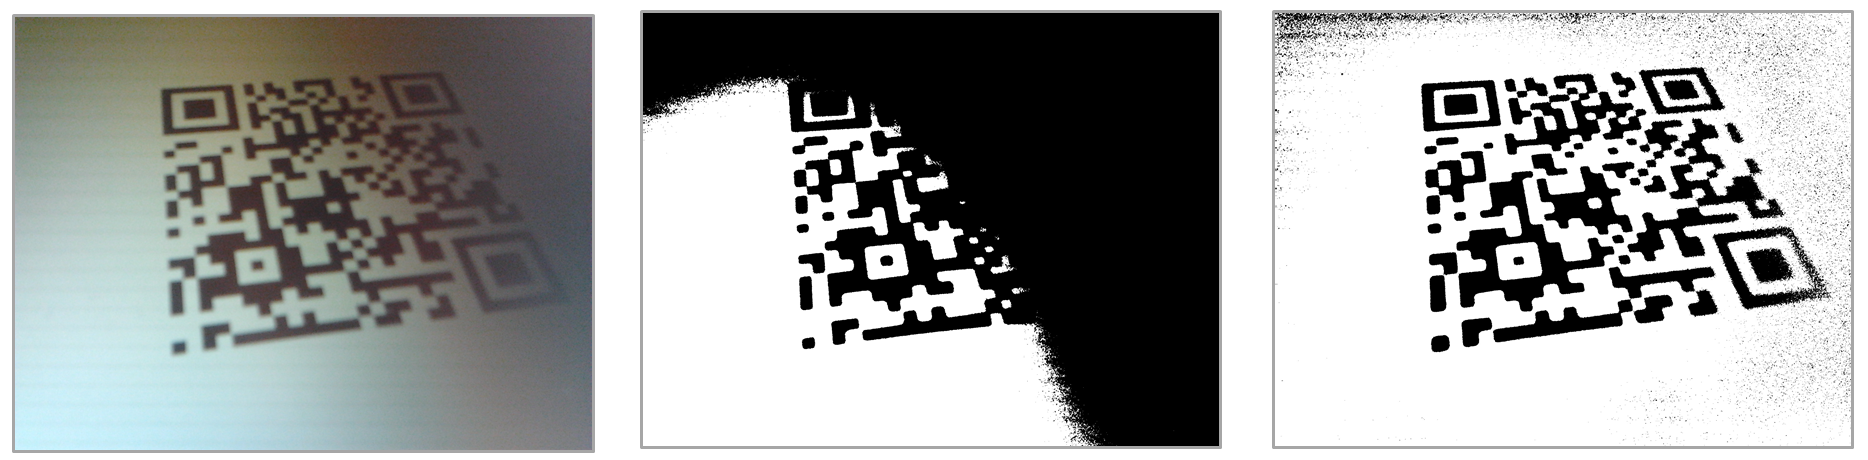
\includegraphics{fig/GlobalAdaptiveThresholdingComparision.PNG}
    }
    \caption{Porovnání globálního (uprostřed) a adaptivního prahování (vpravo)}
    \label{GlobalAdaptiveThresholdingComparision}
  \end{center}
\end{figure}

\begin{figure}[H]
  \begin{center}
    \scalebox{0.15}{
      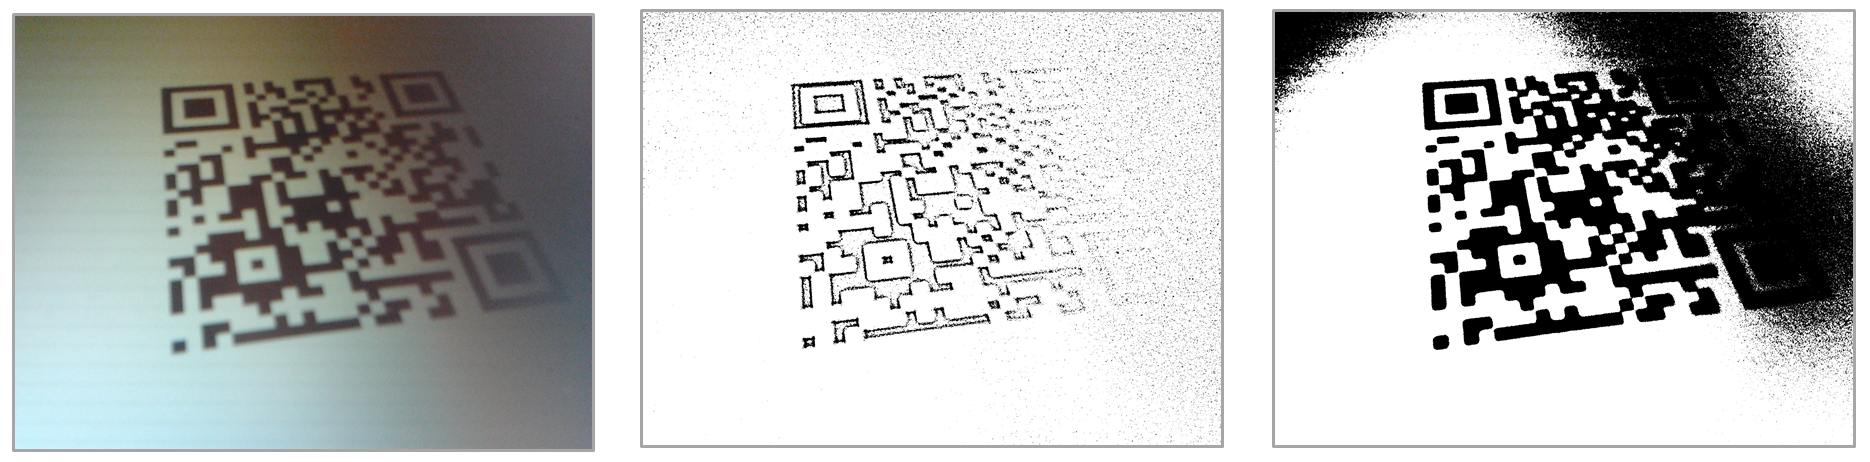
\includegraphics{fig/LocalThresholdingBadSizeOfThresholdBlock.PNG}
    }
    \caption{Výstup prahování při nevhodně zvolené velikost bloku prahování}
    \label{LocalThresholdingBadSizeOfThresholdBlock}
  \end{center}
\end{figure}

\begin{figure}[H]
  \begin{center}
    \scalebox{0.15}{
      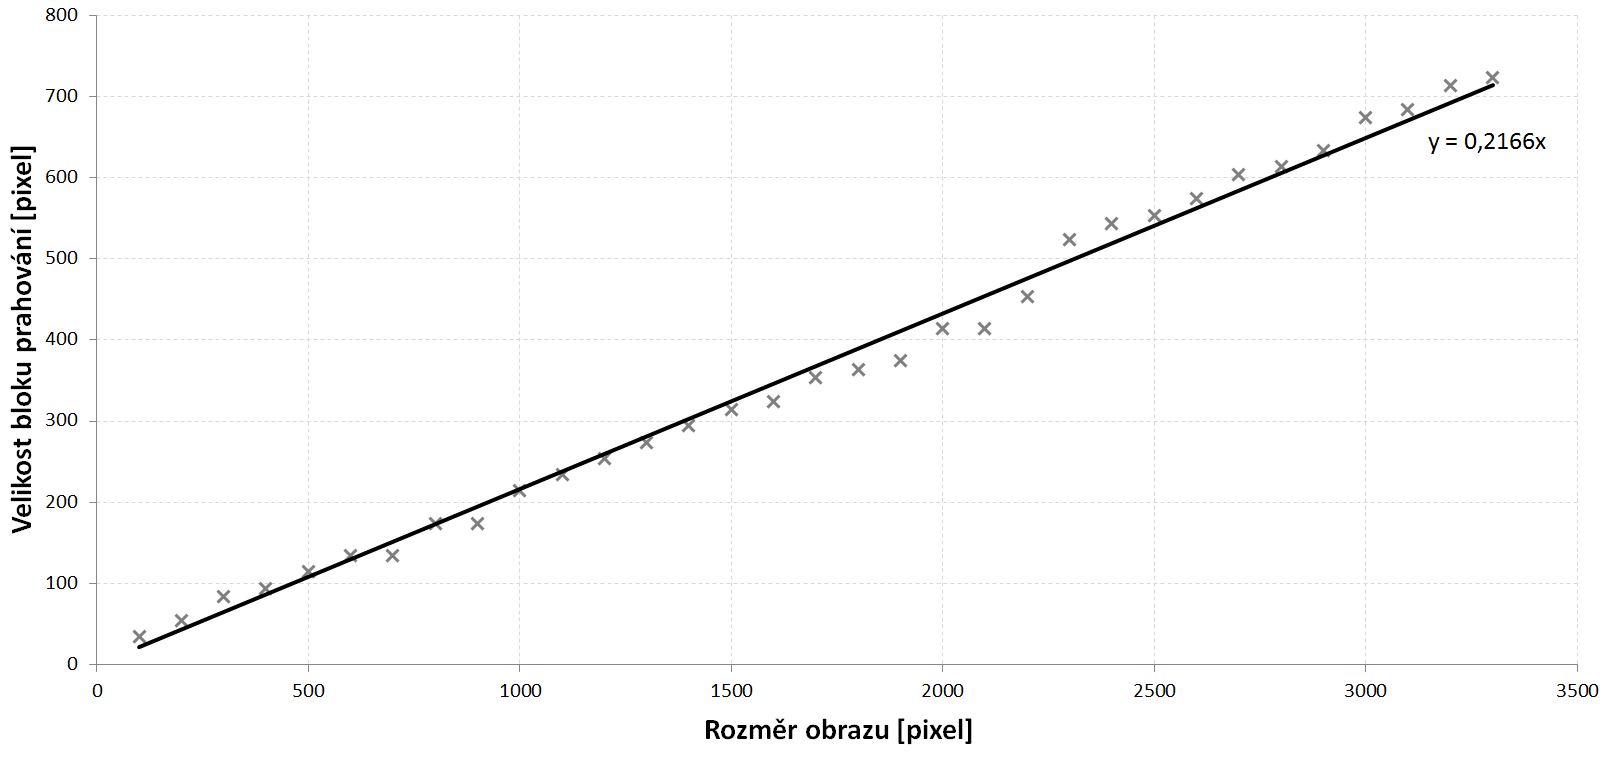
\includegraphics{fig/DependencyOfSizeOfThresholdBlockToQRCodeSizes.PNG}
    }
    \caption{Graf zavislosti vhodné velikosti bloku prahování na rozměrech QR
    kódu}
    \label{DependencyOfSizeOfThresholdBlockToQRCodeSizes}
  \end{center}
\end{figure}

\begin{figure}[H]
  \begin{center}
    \scalebox{0.15}{
      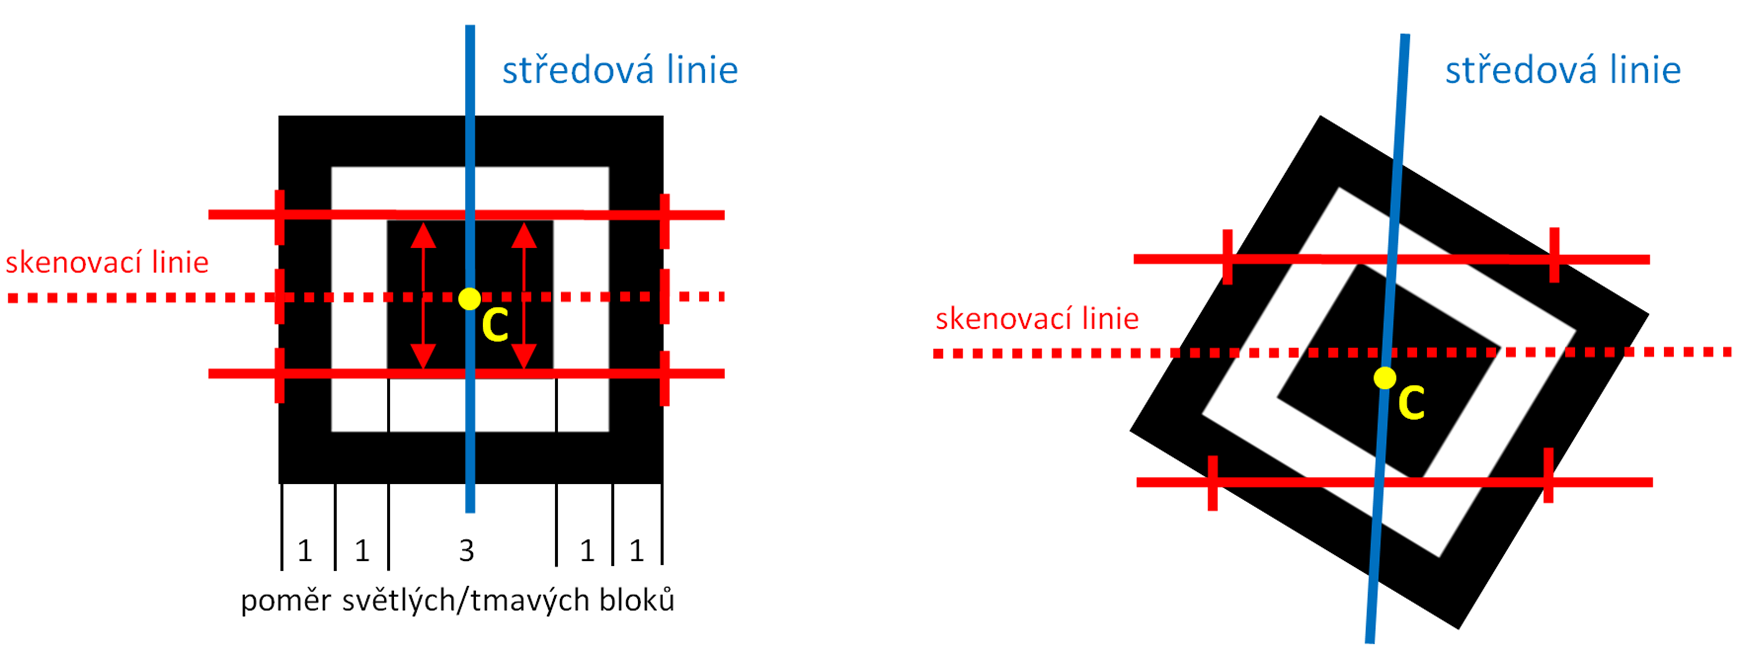
\includegraphics{fig/QRCodeDetectionWithScanline.PNG}
    }
    \caption{Detekce poziční značky pomocí skenovací linky}
    \label{QRCodeDetectionWithScanline}
  \end{center}
\end{figure}

\begin{figure}[H]
  \begin{center}
    \scalebox{0.15}{
      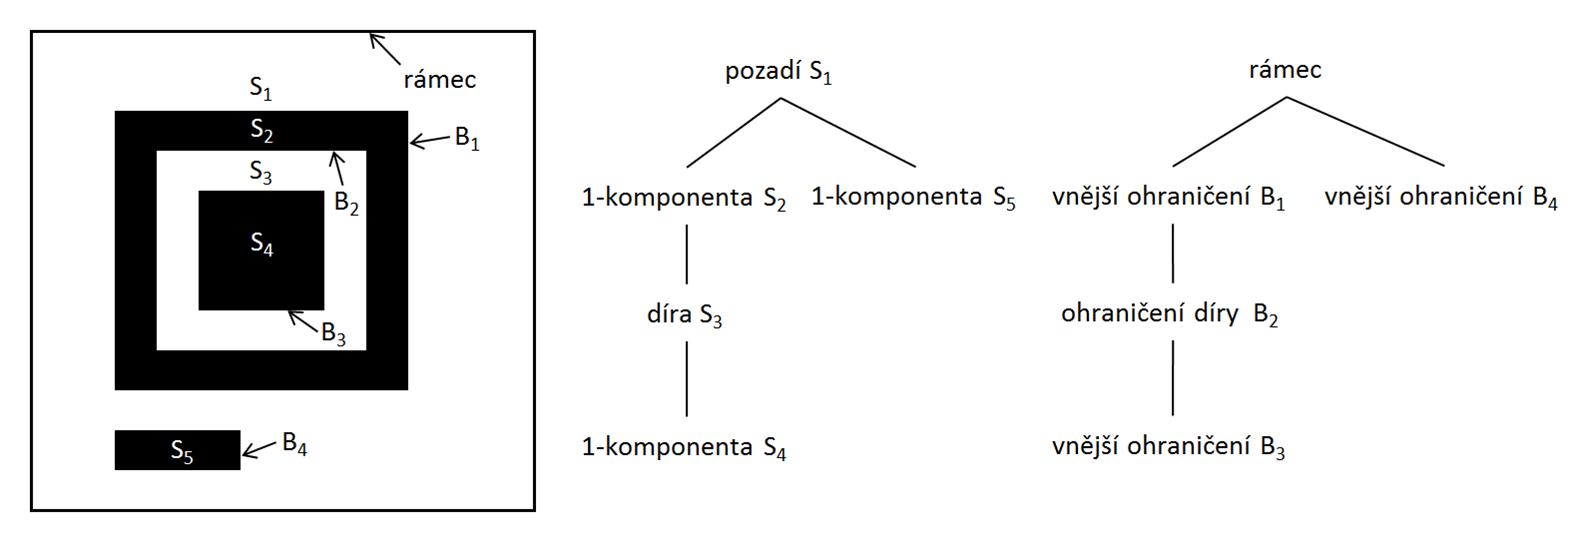
\includegraphics{fig/ContourTopology.PNG}
    }
    \caption{Výstup nálezu kontur a sestavení topologické závislosti mezi nima}
    \label{ContourTopology}
  \end{center}
\end{figure}

\begin{figure}[H]
  \begin{center}
    \scalebox{0.15}{
      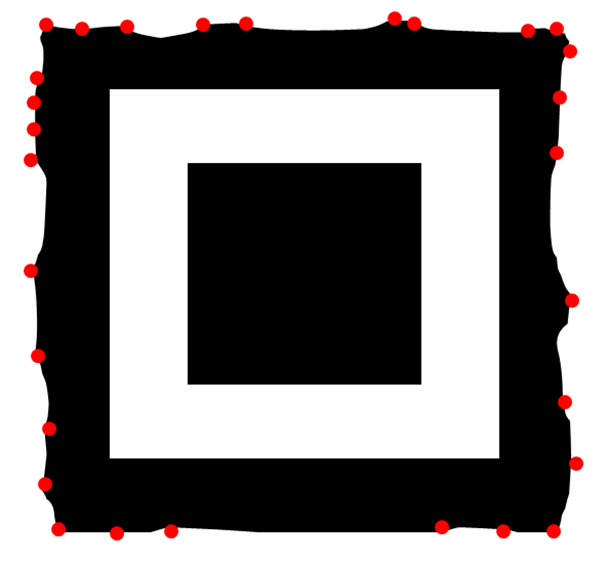
\includegraphics{fig/FinderMarkContourDetection.PNG}
    }
    \caption{Předpokládaný interpolovaný výstup bodů hledání kontury pro
    poziční značku}
    \label{FinderMarkContourDetection}
  \end{center}
\end{figure}

\begin{figure}[H]
  \begin{center}
    \scalebox{0.15}{
      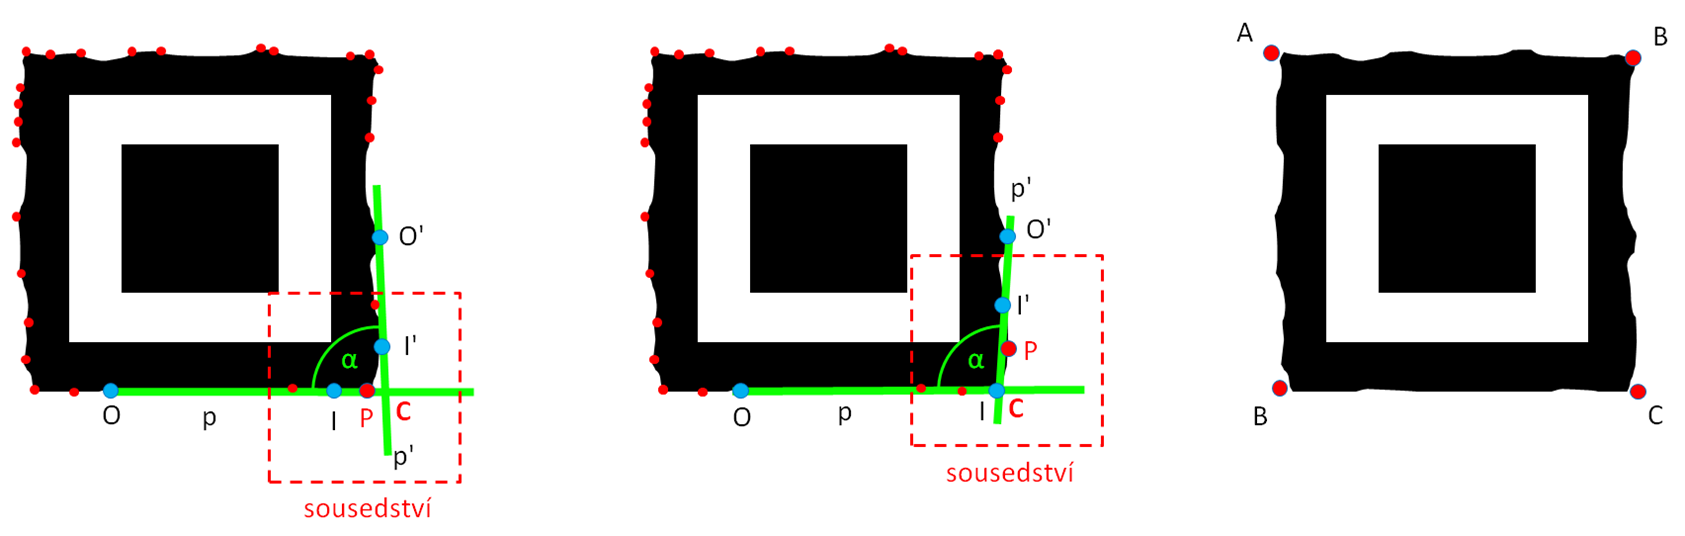
\includegraphics{fig/SearchCornersOfPolygonAlgorithm.PNG}
    }
    \caption{Výstup algoritmu hledání rohů polygonu (zde poziční značky)}
    \label{SearchCornersOfPolygonAlgorithm}
  \end{center}
\end{figure}

\begin{figure}[H]
  \begin{center}
    \scalebox{0.15}{
      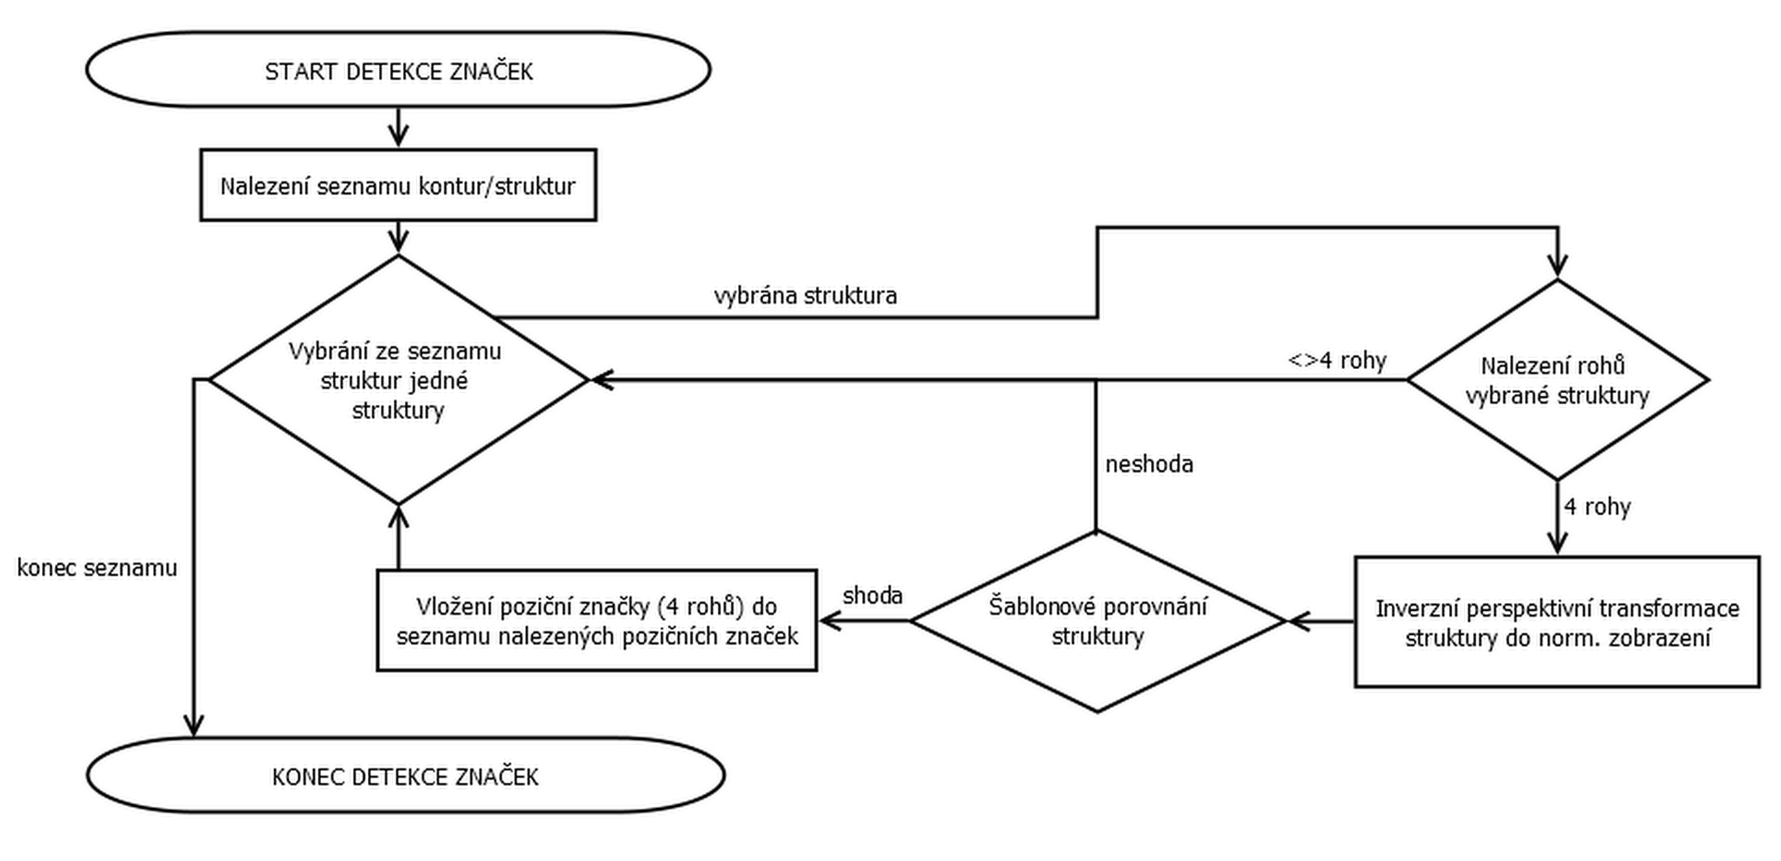
\includegraphics{fig/QRCodeDetectionProcess.PNG}
    } 
    \caption{Proces detekce pozičních značek QR kódu}
    \label{QRCodeDetectionProcess}
  \end{center}
\end{figure}

\begin{figure}[H]
  \begin{center}
    \scalebox{0.15}{
      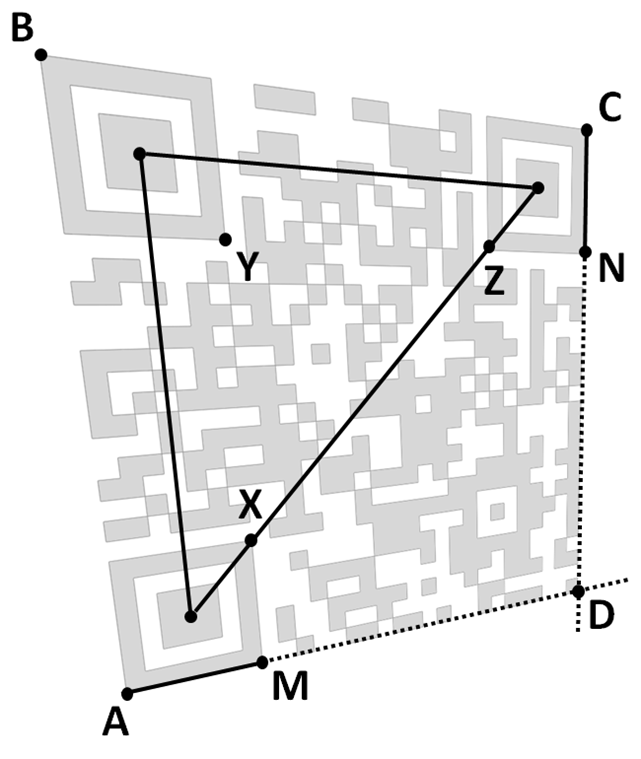
\includegraphics{fig/QRCodeArea.PNG}
    } 
    \caption{Znázornění postupu zjištění čtyř bodů pro inverzní perspektivní
    transformaci}
    \label{QRCodeArea}
  \end{center}
\end{figure}

\begin{figure}[H]
  \begin{center}
    \scalebox{0.15}{
      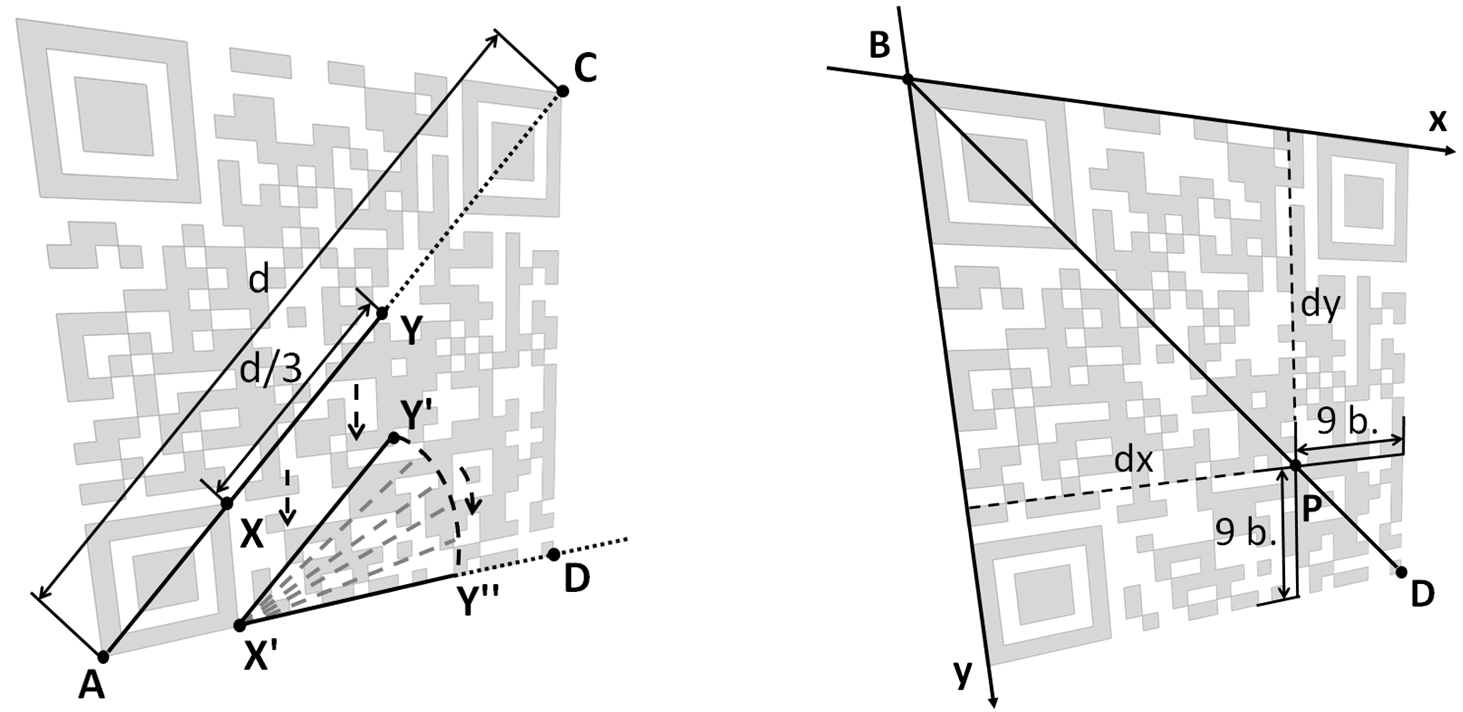
\includegraphics{fig/DeterminingTheFourthPointForTransformation.PNG}
    } 
    \caption{Zjištění 4. bodu vzorkováním (vlevo) a pomocí zarovnávací značky
    (vpravo)}
    \label{DeterminingTheFourthPointForTransformation}
  \end{center}
\end{figure}

\begin{figure}[H]
  \begin{center}
    \scalebox{0.15}{
      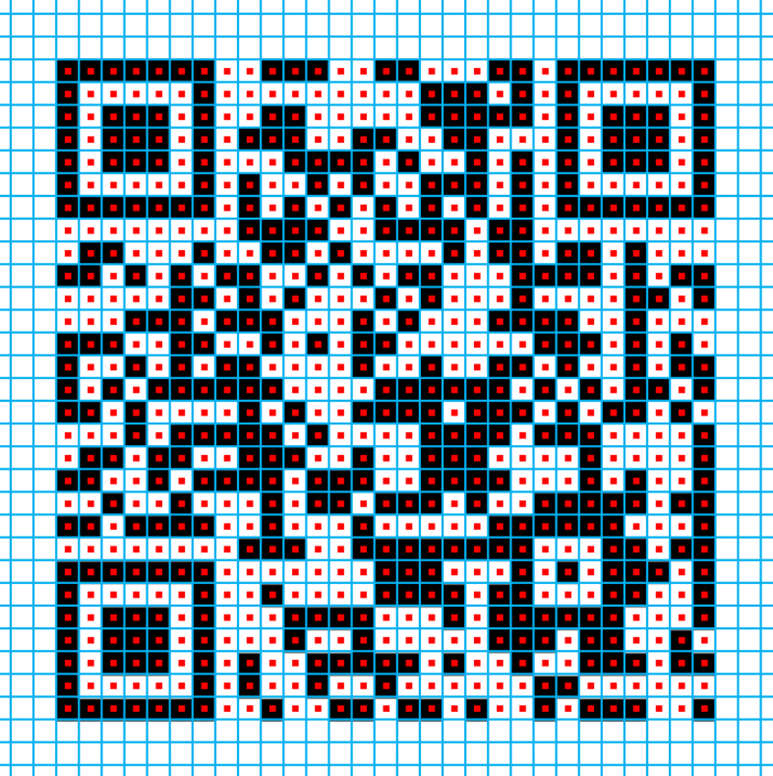
\includegraphics{fig/SamplingGrid.PNG}
    } 
    \caption{Ustanovené vzorkovací mřížky nad QR kódem a oblastí vzorkování
    (červená barva)}
    \label{SamplingGrid}
  \end{center}
\end{figure}

\begin{figure}[H]
  \begin{center}
    \scalebox{0.15}{
      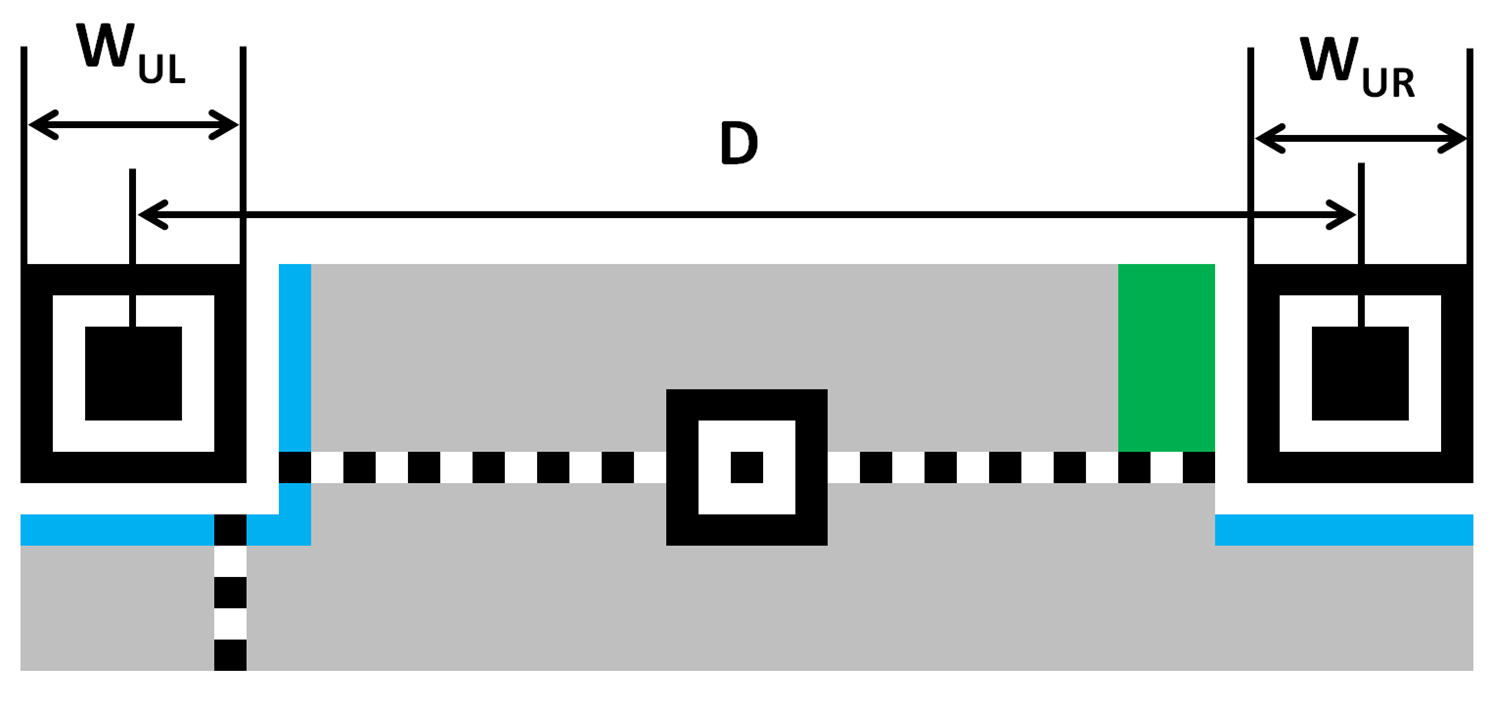
\includegraphics{fig/DeterminingTheVersionOfQRCode.PNG}
    } 
    \caption{Zjištění dočasné verze QR kódu podle jeho rozměrů}
    \label{DeterminingTheVersionOfQRCode}
  \end{center}
\end{figure}

\begin{figure}[H]
  \begin{center}
    \scalebox{0.15}{
      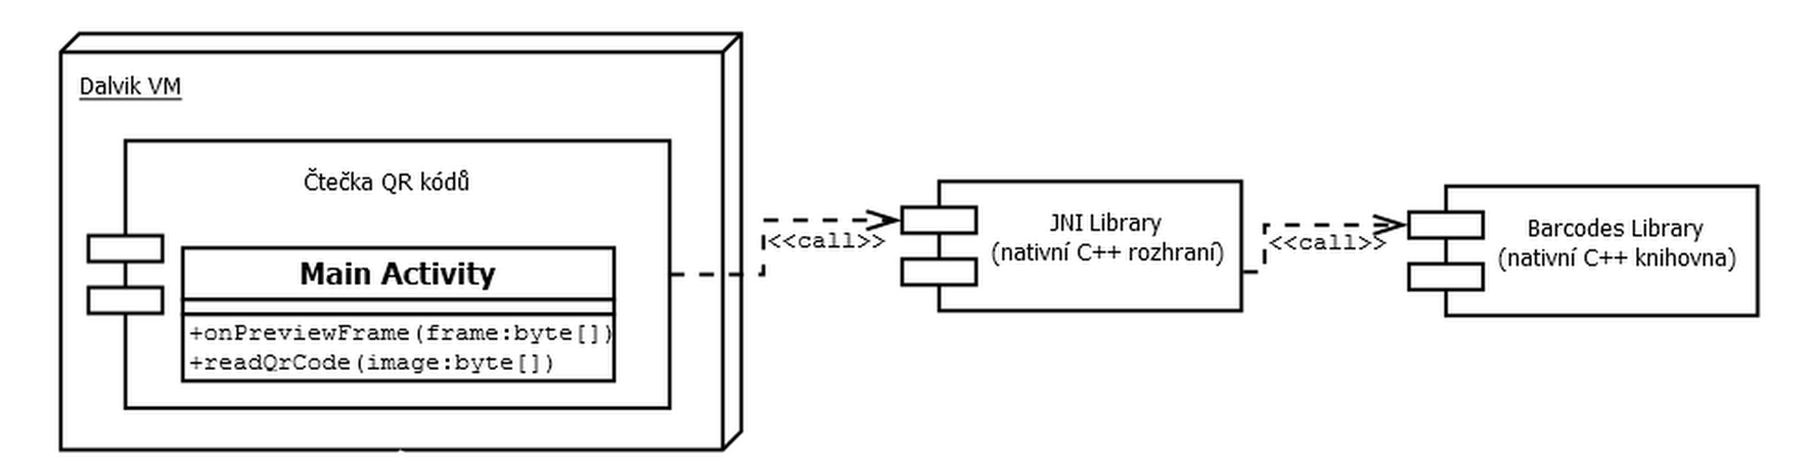
\includegraphics{fig/QRReaderApplicationLibraryDependency.PNG}
    } 
    \caption{Knihovní závislosti aplikace čtečky QR kódů}
    \label{QRReaderApplicationLibraryDependency}
  \end{center}
\end{figure}

\begin{figure}[H]
  \begin{center}
    \scalebox{0.15}{
      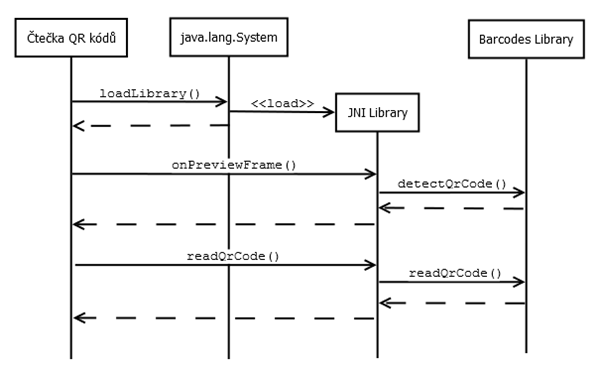
\includegraphics{fig/QRReaderApplicationNativeCalls.PNG}
    } 
    \caption{Sekvenční diagram znázorňující volání funkcí nativního rozhraní}
    \label{QRReaderApplicationNativeCalls}
  \end{center}
\end{figure}

\begin{equation}
  I = 0,299R + 0,587G + 0,114B
\end{equation}

\begin{equation}
  p_{dst} = \mathbf{H} p_{src}
\end{equation}

\begin{equation}
  \left(
    \begin{array}{c}
      x w \\
      y w \\
      w \\
    \end{array}
  \right)
  =
  \left(
    \begin{array}{ccc}
      p_{1} & p_{2}  & p_{3} \\
      p_{4} & p_{5}  & p_{6} \\
      p_{7} & p_{8}  & p_{9} \\
    \end{array}
  \right)
  \left(
    \begin{array}{c}
      X \\
      Y \\
      1 \\
    \end{array}
  \right)
\end{equation}

\begin{equation}
  \mathbf{A} \vec{p} =
  \left(
    \begin{array}{ccccccccc}
      X_{1} & Y_{1} & 1 & 0 & 0 & 0 & -X_{1} x_{1} & -Y_{1} x_{1} & x_{1} \\
      0 & 0 & 0 & X_{1} & Y_{1} & 1 & -X_{1} y_{1} & -Y_{1} y_{1} & y_{1} \\
      X_{2} & Y_{2} & 1 & 0 & 0 & 0 & -X_{2} x_{2} & -Y_{2} x_{2} & x_{2} \\
      0 & 0 & 0 & X_{2} & Y_{2} & 1 & -X_{2} y_{2} & -Y_{2} y_{2} & y_{2} \\
      X_{3} & Y_{3} & 1 & 0 & 0 & 0 & -X_{3} x_{3} & -Y_{3} x_{3} & x_{3} \\
      0 & 0 & 0 & X_{3} & Y_{3} & 1 & -X_{3} y_{3} & -Y_{3} y_{3} & y_{3} \\
      X_{4} & Y_{4} & 1 & 0 & 0 & 0 & -X_{4} x_{4} & -Y_{4} x_{4} & x_{4} \\
      0 & 0 & 0 & X_{4} & Y_{4} & 1 & -X_{4} y_{4} & -Y_{4} y_{4} & y_{4} \\
    \end{array}
  \right)
  \left(
    \begin{array}{c}
      p_{1} \\
      p_{2} \\
      p_{3} \\
      p_{4} \\
      p_{5} \\
      p_{6} \\
      p_{7} \\
      p_{8} \\
      p_{9} \\
    \end{array}
  \right)
  = 0
\end{equation}

\begin{eqnarray}
  D = \bigg[ B_{x} + \frac{dx}{s}(s + 9) ; B_{y} + \frac{dy}{s}(s + 9) \bigg] \\
  dx = P_{x} - B_{x} \quad dy = P_{y} - B_{y}
\end{eqnarray}

\begin{equation}
  V = \frac{7 D}{2 (W_{UL} + W_{UR})} - 2,5
\end{equation}
\chapter{Implementace}
\chapter{Testování a ?? rozšíření}
\chapter{Závěr}






\chapter{Úvod}
Abychom mohli napsat odborný text jasně a~srozumitelně, musíme splnit několik základních předpokladů:
\begin{itemize}
\item Musíme mít co říci,
\item musíme vědět, komu to chceme říci,
\item musíme si dokonale promyslet obsah,
\item musíme psát strukturovaně. 
\end{itemize}

Tyto a další pokyny jsou dostupné též na školních internetových stránkách \cite{fitWeb}.

Přehled základů typografie a tvorby dokumentů s využitím systému \LaTeX je 
uveden v~\cite{Rybicka}.

\section{Musíme mít co říci}
Dalším důležitým předpokladem dobrého psaní je {\it psát pro někoho}. Píšeme-li si poznámky sami pro sebe, píšeme je jinak než výzkumnou zprávu, článek, diplomovou práci, knihu nebo dopis. Podle předpokládaného čtenáře se rozhodneme pro způsob psaní, rozsah informace a~míru detailů.

\section{Musíme vědět, komu to chceme říci}
Dalším důležitým předpokladem dobrého psaní je psát pro někoho. Píšeme-li si poznámky sami pro sebe, píšeme je jinak než výzkumnou zprávu, článek, diplomovou práci, knihu nebo dopis. Podle předpokládaného čtenáře se rozhodneme pro způsob psaní, rozsah informace a~míru detailů.

\section{Musíme si dokonale promyslet obsah}
Musíme si dokonale promyslet a~sestavit obsah sdělení a~vytvořit pořadí, v~jakém chceme čtenáři své myšlenky prezentovat. 
Jakmile víme, co chceme říci a~komu, musíme si rozvrhnout látku. Ideální je takové rozvržení, které tvoří logicky přesný a~psychologicky stravitelný celek, ve kterém je pro všechno místo a~jehož jednotlivé části do sebe přesně zapadají. Jsou jasné všechny souvislosti a~je zřejmé, co kam patří.

Abychom tohoto cíle dosáhli, musíme pečlivě organizovat látku. Rozhodneme, co budou hlavní kapitoly, co podkapitoly a~jaké jsou mezi nimi vztahy. Diagramem takové organizace je graf, který je velmi podobný stromu, ale ne řetězci. Při organizaci látky je stejně důležitá otázka, co do osnovy zahrnout, jako otázka, co z~ní vypustit. Příliš mnoho podrobností může čtenáře právě tak odradit jako žádné detaily.

Výsledkem této etapy je osnova textu, kterou tvoří sled hlavních myšlenek a~mezi ně zařazené detaily.

\section{Musíme psát strukturovaně} 
Musíme začít psát strukturovaně a~současně pracujeme na co nejsrozumitelnější formě, včetně dobrého slohu a~dokonalého značení. 
Máme-li tedy myšlenku, představu o~budoucím čtenáři, cíl a~osnovu textu, můžeme začít psát. Při psaní prvního konceptu se snažíme zaznamenat všechny své myšlenky a~názory vztahující se k~jednotlivým kapitolám a~podkapitolám. Každou myšlenku musíme vysvětlit, popsat a~prokázat. Hlavní myšlenku má vždy vyjadřovat hlavní věta a~nikoliv věta vedlejší.

I k~procesu psaní textu přistupujeme strukturovaně. Současně s~tím, jak si ujasňujeme strukturu písemné práce, vytváříme kostru textu, kterou postupně doplňujeme. Využíváme ty prostředky DTP programu, které podporují strukturovanou stavbu textu (předdefinované typy pro nadpisy a~bloky textu). 


\chapter{Několik formálních pravidel}
Naším cílem je vytvořit jasný a~srozumitelný text. Vyjadřujeme se proto přesně, píšeme dobrou češtinou (nebo zpravidla angličtinou) a~dobrým slohem podle obecně přijatých zvyklostí. Text má upravit čtenáři cestu k~rychlému pochopení problému, předvídat jeho obtíže a~předcházet jim. Dobrý sloh předpokládá bezvadnou gramatiku, správnou interpunkci a~vhodnou volbu slov. Snažíme se, aby náš text nepůsobil příliš jednotvárně používáním malého výběru slov a~tím, že některá zvlášť oblíbená slova používáme příliš často. Pokud používáme cizích slov, je samozřejmým předpokladem, že známe jejich přesný význam. Ale i~českých slov musíme používat ve správném smyslu. Např. platí jistá pravidla při používání slova {\it zřejmě}. Je {\it zřejmé} opravdu zřejmé? A~přesvědčili jsme se, zda to, co je {\it zřejmé} opravdu platí? Pozor bychom si měli dát i~na příliš časté používání zvratného se. Například obratu {\it dokázalo se}, že... zásadně nepoužíváme. Není špatné používat autorského {\it my}, tím předpokládáme, že něco řešíme, nebo například zobecňujeme spolu se čtenářem. V~kvalifikačních pracích použijeme autorského {\it já} (například když vymezujeme podíl vlastní práce vůči převzatému textu), ale v~běžném textu se nadměrné používání první osoby jednotného čísla nedoporučuje.

Za pečlivý výběr stojí i~symbolika, kterou používáme ke {\it značení}. Máme tím na mysli volbu zkratek a~symbolů používaných například pro vyjádření typů součástek, pro označení hlavních činností programu, pro pojmenování ovládacích kláves na klávesnici, pro pojmenování proměnných v~matematických formulích a~podobně. Výstižné a~důsledné značení může čtenáři při četbě textu velmi pomoci. Je vhodné uvést seznam značení na začátku textu. Nejen ve značení, ale i~v~odkazech a~v~celkové tiskové úpravě je důležitá důslednost.

S tím souvisí i~pojem z~typografie nazývaný {\it vyznačování}. Zde máme na mysli způsob sazby textu pro jeho zvýraznění. Pro zvolené značení by měl být zvolen i~způsob vyznačování v~textu. Tak například klávesy mohou být umístěny do obdélníčku, identifikátory ze zdrojového textu mohou být vypisovány {\tt písmem typu psací stroj} a~podobně.

Uvádíme-li některá fakta, neskrýváme jejich původ a~náš vztah k~nim. Když něco tvrdíme, vždycky výslovně uvedeme, co z~toho bylo dokázáno, co teprve bude dokázáno v~našem textu a~co přebíráme z~literatury s~uvedením odkazu na příslušný zdroj. V~tomto směru nenecháváme čtenáře nikdy na pochybách, zda jde o~myšlenku naši nebo převzatou z~literatury.

Nikdy neplýtváme čtenářovým časem výkladem triviálních a~nepodstatných informací. Neuvádíme rovněž několikrát totéž jen jinými slovy. Při pozdějších úpravách textu se nám může některá dříve napsaná pasáž jevit jako zbytečně podrobná nebo dokonce zcela zbytečná. Vypuštění takové pasáže nebo alespoň její zestručnění přispěje k~lepší čitelnosti práce! Tento krok ale vyžaduje odvahu zahodit čas, který jsme jejímu vytvoření věnovali. 


\chapter{Nikdy to nebude naprosto dokonalé}
Když jsme už napsali vše, o~čem jsme přemýšleli, uděláme si den nebo dva dny volna a~pak si přečteme sami rukopis znovu. Uděláme ještě poslední úpravy a~skončíme. Jsme si vědomi toho, že vždy zůstane něco nedokončeno, vždy existuje lepší způsob, jak něco vysvětlit, ale každá etapa úprav musí být konečná.


\chapter{Typografické a~jazykové zásady}
Při tisku odborného textu typu {\it technická zpráva} (anglicky {\it technical report}), ke kterému patří například i~text kvalifikačních prací, se často volí formát A4 a~často se tiskne pouze po jedné straně papíru. V~takovém případě volte levý okraj všech stránek o~něco větší než pravý -- v~tomto místě budou papíry svázány a~technologie vazby si tento požadavek vynucuje. Při vazbě s~pevným hřbetem by se levý okraj měl dělat o~něco širší pro tlusté svazky, protože se stránky budou hůře rozevírat a~levý okraj se tak bude oku méně odhalovat.

Horní a~spodní okraj volte stejně veliký, případně potištěnou část posuňte mírně nahoru (horní okraj menší než dolní). Počítejte s~tím, že při vazbě budou okraje mírně oříznuty.

Pro sazbu na stránku formátu A4 je vhodné používat pro základní text písmo stupně (velikosti) 11 bodů. Volte šířku sazby 15 až 16 centimetrů a~výšku 22 až 23 centimetrů (včetně případných hlaviček a~patiček). Proklad mezi řádky se volí 120 procent stupně použitého základního písma, což je optimální hodnota pro rychlost čtení souvislého textu. V~případě použití systému LaTeX ponecháme implicitní nastavení. Při psaní kvalifikační práce se řiďte příslušnými závaznými požadavky.

Stupeň písma u~nadpisů různé úrovně volíme podle standardních typografických pravidel. 
Pro všechny uvedené druhy nadpisů se obvykle používá polotučné nebo tučné písmo (jednotně buď všude polotučné nebo všude tučné). Proklad se volí tak, aby se následující text běžných odstavců sázel pokud možno na {\it pevný rejstřík}, to znamená jakoby na linky s~předem definovanou a~pevnou roztečí.

Uspořádání jednotlivých částí textu musí být přehledné a~logické. Je třeba odlišit názvy kapitol a~podkapitol -- píšeme je malými písmeny kromě velkých začátečních písmen. U~jednotlivých odstavců textu odsazujeme první řádek odstavce asi o~jeden až dva čtverčíky (vždy o~stejnou, předem zvolenou hodnotu), tedy přibližně o~dvě šířky velkého písmene M základního textu. Poslední řádek předchozího odstavce a~první řádek následujícího odstavce se v~takovém případě neoddělují svislou mezerou. Proklad mezi těmito řádky je stejný jako proklad mezi řádky uvnitř odstavce.

Při vkládání obrázků volte jejich rozměry tak, aby nepřesáhly oblast, do které se tiskne text (tj. okraje textu ze všech stran). Pro velké obrázky vyčleňte samostatnou stránku. Obrázky nebo tabulky o~rozměrech větších než A4 umístěte do písemné zprávy formou skládanky všité do přílohy nebo vložené do záložek na zadní desce.

Obrázky i~tabulky musí být pořadově očíslovány. Číslování se volí buď průběžné v~rámci celého textu, nebo -- což bývá praktičtější -- průběžné v~rámci kapitoly. V~druhém případě se číslo tabulky nebo obrázku skládá z~čísla kapitoly a~čísla obrázku/tabulky v~rámci kapitoly -- čísla jsou oddělena tečkou. Čísla podkapitol nemají na číslování obrázků a~tabulek žádný vliv.

Tabulky a~obrázky používají své vlastní, nezávislé číselné řady. Z toho vyplývá, že v~odkazech uvnitř textu musíme kromě čísla udat i~informaci o~tom, zda se jedná o~obrázek či tabulku (například ``... {\it viz tabulka 2.7} ...''). Dodržování této zásady je ostatně velmi přirozené.

Pro odkazy na stránky, na čísla kapitol a~podkapitol, na čísla obrázků a~tabulek a~v~dalších podobných příkladech využíváme speciálních prostředků DTP programu, které zajistí vygenerování správného čísla i~v~případě, že se text posune díky změnám samotného textu nebo díky úpravě parametrů sazby. Příkladem takového prostředku v~systému LaTeX je odkaz na číslo odpovídající umístění značky v~textu, například návěští ($\backslash${\tt ref\{navesti\}} -- podle umístění návěští se bude jednat o~číslo kapitoly, podkapitoly, obrázku, tabulky nebo podobného číslovaného prvku), na stránku, která obsahuje danou značku ($\backslash${\tt pageref\{navesti\}}), nebo na literární odkaz ($\backslash${\tt cite\{identifikator\}}).

Rovnice, na které se budeme v~textu odvolávat, opatříme pořadovými čísly při pravém okraji příslušného řádku. Tato pořadová čísla se píší v~kulatých závorkách. Číslování rovnic může být průběžné v~textu nebo v~jednotlivých kapitolách.

Jste-li na pochybách při sazbě matematického textu, snažte se dodržet způsob sazby definovaný systémem LaTeX. Obsahuje-li vaše práce velké množství matematických formulí, doporučujeme dát přednost použití systému LaTeX.

Mezeru neděláme tam, kde se spojují číslice s~písmeny v~jedno slovo nebo v~jeden znak -- například {\it 25krát}.

Členicí (interpunkční) znaménka tečka, čárka, středník, dvojtečka, otazník a~vykřičník, jakož i~uzavírací závorky a~uvozovky se přimykají k~předcházejícímu slovu bez mezery. Mezera se dělá až za nimi. To se ovšem netýká desetinné čárky (nebo desetinné tečky). Otevírací závorka a~přední uvozovky se přimykají k~následujícímu slovu a~mezera se vynechává před nimi -- (takto) a~``takto''.

Pro spojovací a~rozdělovací čárku a~pomlčku nepoužíváme stejný znak. Pro pomlčku je vyhrazen jiný znak (delší). V~systému TeX (LaTeX) se spojovací čárka zapisuje jako jeden znak ``pomlčka'' (například ``Brno-město''), pro sázení textu ve smyslu intervalu nebo dvojic, soupeřů a~podobně se ve zdrojovém textu používá dvojice znaků ``pomlčka'' (například ``zápas Sparta -- Slavie''; ``cena 23--25 korun''), pro výrazné oddělení části věty, pro výrazné oddělení vložené věty, pro vyjádření nevyslovené myšlenky a~v~dalších situacích (viz Pravidla českého pravopisu) se používá nejdelší typ pomlčky, která se ve zdrojovém textu zapisuje jako trojice znaků ``pomlčka'' (například ``Další pojem --- jakkoliv se může zdát nevýznamný --- bude neformálně definován v~následujícím odstavci.''). Při sazbě matematického mínus se při sazbě používá rovněž odlišný znak. V~systému TeX je ve zdrojovém textu zapsán jako normální mínus (tj. znak ``pomlčka''). Sazba v~matematickém prostředí, kdy se vzoreček uzavírá mezi dolary, zajistí vygenerování správného výstupu.

Lomítko se píše bez mezer. Například školní rok 2008/2009.

Pravidla pro psaní zkratek jsou uvedena v~Pravidlech českého pravopisu \cite{Pravidla}. I~z~jiných důvodů je vhodné, abyste tuto knihu měli po ruce. 


\section{Co to je normovaná stránka?}
Pojem {\it normovaná stránka} se vztahuje k~posuzování objemu práce, nikoliv k~počtu vytištěných listů. Z historického hlediska jde o~počet stránek rukopisu, který se psal psacím strojem na speciální předtištěné formuláře při dodržení průměrné délky řádku 60 znaků a~při 30 řádcích na stránku rukopisu. Vzhledem k~zápisu korekturních značek se používalo řádkování 2 (ob jeden řádek). Tyto údaje (počet znaků na řádek, počet řádků a~proklad mezi nimi) se nijak nevztahují ke konečnému vytištěnému výsledku. Používají se pouze pro posouzení rozsahu. Jednou normovanou stránkou se tedy rozumí 60*30 = 1800 znaků. Obrázky zařazené do textu se započítávají do rozsahu písemné práce odhadem jako množství textu, které by ve výsledném dokumentu potisklo stejně velkou plochu.

Orientační rozsah práce v~normostranách lze v~programu Microsoft Word zjistit pomocí funkce {\it Počet slov} v~menu {\it Nástroje}, když hodnotu {\it Znaky (včetně mezer)} vydělíte konstantou 1800. Do rozsahu práce se započítává pouze text uvedený v~jádru práce. Části jako abstrakt, klíčová slova, prohlášení, obsah, literatura nebo přílohy se do rozsahu práce nepočítají. Je proto nutné nejdříve označit jádro práce a~teprve pak si nechat spočítat počet znaků. Přibližný rozsah obrázků odhadnete ručně. Podobně lze postupovat i~při použití OpenOffice. Při použití systému LaTeX pro sazbu je situace trochu složitější. Pro hrubý odhad počtu normostran lze využít součet velikostí zdrojových souborů práce podělený konstantou cca 2000 (normálně bychom dělili konstantou 1800, jenže ve zdrojových souborech jsou i~vyznačovací příkazy, které se do rozsahu nepočítají). Pro přesnější odhad lze pak vyextrahovat holý text z~PDF (např. metodou cut-and-paste nebo {\it Save as Text...}) a~jeho velikost podělit konstantou 1800. 


\chapter{Závěr}
Závěrečná kapitola obsahuje zhodnocení dosažených výsledků se zvlášť vyznačeným vlastním přínosem studenta. Povinně se zde objeví i zhodnocení z pohledu dalšího vývoje projektu, student uvede náměty vycházející ze zkušeností s řešeným projektem a uvede rovněž návaznosti na právě dokončené projekty.

%=========================================================================
